\ylDisplay{Must kast} % Ülesande nimi
{Tundmatu autor} % Autor
{lõppvoor} % Voor
{2013} % Aasta
{P 5} % Ülesande nr.
{2} % Raskustase
{
% Teema: Elektriõpetus

\ifStatement
Kui joonisel näidatud musta kasti klemmide $A$ ja $B$ külge ühendada patarei pingega $U$ ja klemmide $C$ ja $D$ külge voltmeeter, on voltmeetri näit $U$. Kui ühendada sama patarei klemmide $C$ ja $D$ külge ning voltmeeter klemmide $A$ ja $B$ külge, on voltmeetri näit $U/2$. Teades, et mustas kastis on ainult identsed takistid, joonistage musta kasti skeem!
\begin{center}
	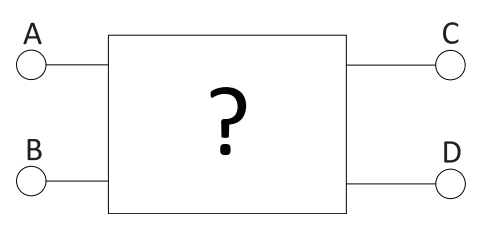
\includegraphics[width=0.5\linewidth]{2013-v3p-05-yl.png}
\end{center}
\fi

\ifHint
Ülesande lahendusel piisab ainult kahe takisti lisamisest süsteemi.
\fi

\ifSolution
Kui klemmide $A$ ja $B$ külge ühendada patarei ja klemmide $C$ ja $D$ külge voltmeeter, siis läbi takisti $R_2$ vool ei lähe; kogu pinge on voltmeetril, mis näitab $U$. Kui aga patarei ühendada klemmide $C$ ja $D$ külge ja voltmeeter klemmide $A$ ja $B$ külge, jaotub pinge $U$ võrdselt takistite $R_1$ ja $R_2$ vahel. Voltmeeter näitab $U/2$.

\begin{center}
	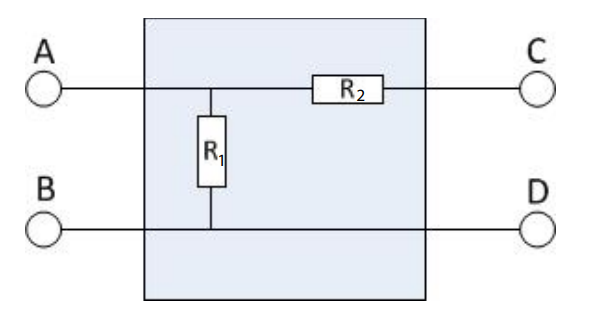
\includegraphics[width=0.5\linewidth]{2013-v3p-05-lah.png}
\end{center}
\fi
}